%%=============================================================================
%% Test set-up
%%=============================================================================

\chapter{Test set-up}%
\label{ch:test_setup}

Dit hoofdstuk biedt een gedetailleerde beschrijving van het proces waarmee de uiteindelijke test set-up tot stand is gekomen. Al de aparte onderdelen worden besproken en vervolgens worden alle componenten samengevoegd tot één werkende test set-up. Elk van de volgende stappen is genoeg gedocumenteerd en kan gemakkelijk gereproduceerd worden door anderen die een vergelijkbare set-up willen maken.

\section{Kalibratie van de sensoren}%
\label{sec:kalibratie}

Om de MQ-sensoren te kalibreren is het zeer belangrijk dat ze voor de eerste keer gebruik een voorverwarmperdiode van 24-48u hebben gehad, hierna volstaat een opwarmperiode van 5 minuten bij elke keer dat ze gebruikt worden. Hierna moet de R\textsubscript{0} waarde voor iedere sensor worden berekent, het is belangrijk dat dit gedaan wordt in schone lucht. In sectie~\ref{sec:hoe-luchtsamenstelling meten} werd getoond hoe de R\textsubscript{0} waarde kan worden berekend. In de Arduino functie in bijlage (~\ref{lst:kalibratie}) is te zien hoe dit gebeurt volgens de werkwijze in sectie~\ref{sec:hoe-luchtsamenstelling meten}.

Nadat dit script enige tijd heeft gedraaid kan R\textsubscript{0} worden bepaald via het gemiddelde te nemen. In figuur~\ref{fig:avg_van_R0} is te zien hoe dit gemakkelijk kan worden gedaan aan de hand van een SQL-tabel.

\begin{figure}[h]
    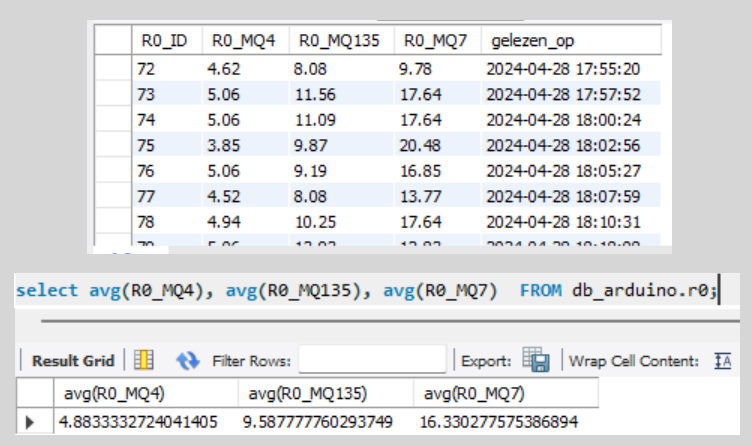
\includegraphics[scale=0.5, center]{avg_van_R0.png}
    \caption[R0 waarden in SQL]{Bepalen van de R0 waarden via SQL}
    \label{fig:avg_van_R0}
\end{figure}

Nu de R\textsubscript{0} waarden zijn bepaald kan er per gas de ppm-waarde worden berekend. In sectie~\ref{sec:hoe-luchtsamenstelling meten} wordt uitgelegd hoe de waarden van de gevoeligheidscurves eerst moeten worden bepaald, en zoals reeds aangehaald wordt dit het best gedaan via een tool zoals WebPlotDigitizer
%TODO bron webplotdigitizer
. Hier kan een grafiek worden ingeladen waarna de x- en y-as moeten worden uitgelijnd, het is belangrijk dat deze assen worden ingesteld als logaritmisch (zie figuur~\ref{fig:x_en_y}). Vervolgens moeten er per gas 2 punten worden aangeduid, die liefst zo ver mogelijk van elkaar liggen (figuur~\ref{fig:voorbeeld}).

\begin{figure}[h]
    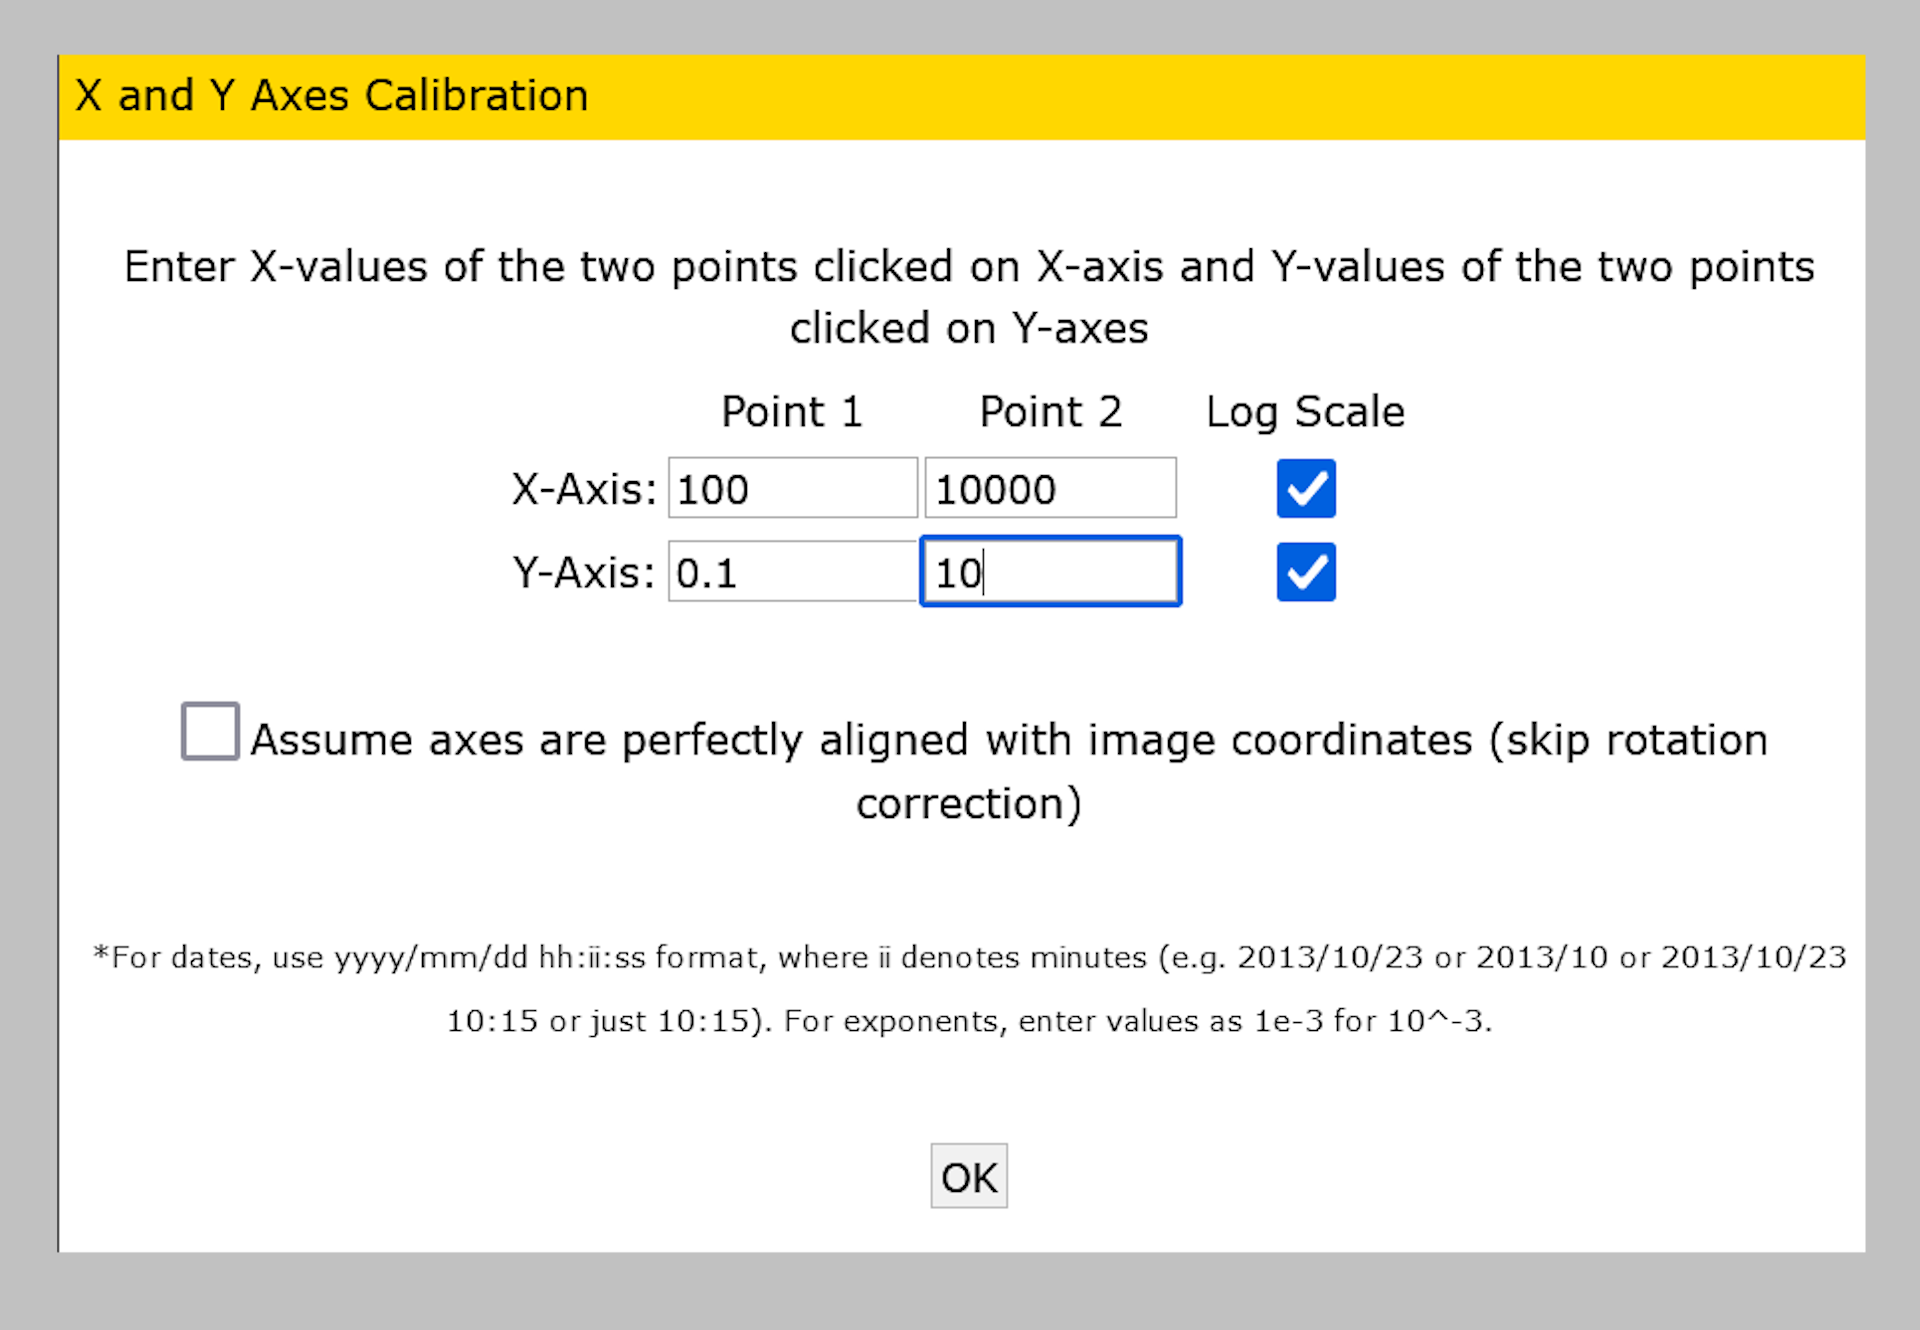
\includegraphics[scale=0.25, center]{XenY.png}
    \caption[Uitlijnen X- en Y-assen]{Uitlijnen van de X- en Y-assen in WebPlotDigitizer}
    \label{fig:x_en_y}
\end{figure}

\begin{figure}[h]
    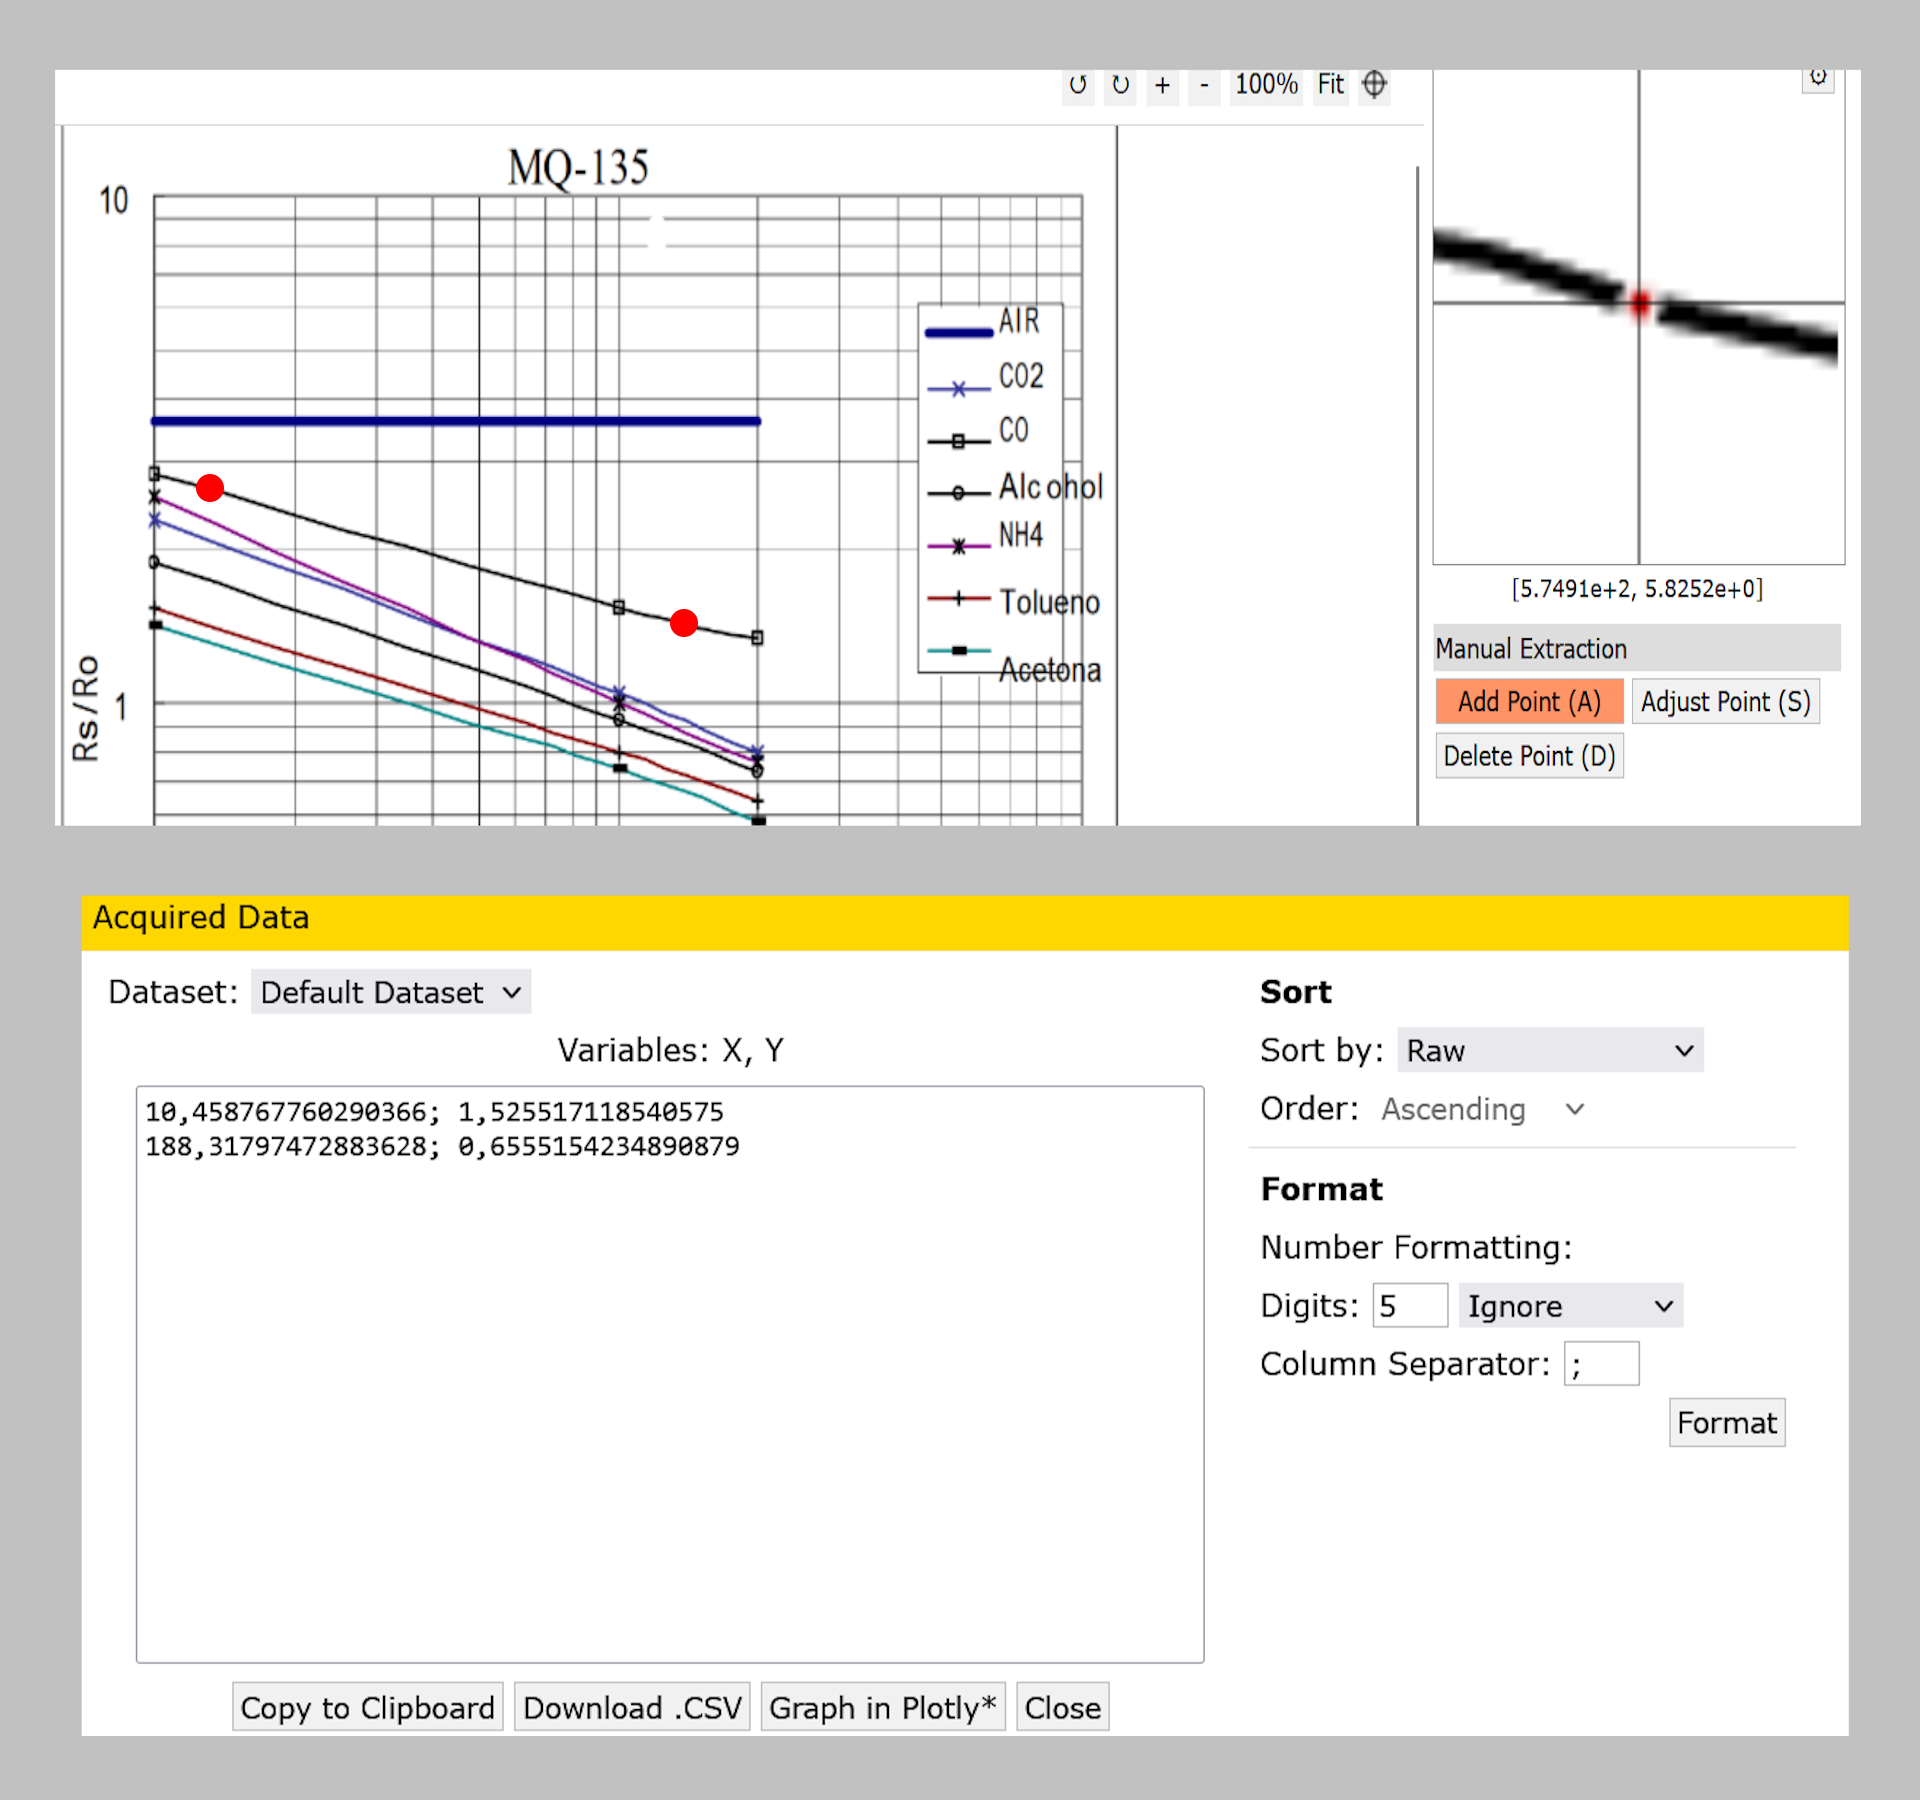
\includegraphics[scale=0.25, center]{voorbeeld.png}
    \caption[Datapunten uit WebPlotDigitizer]{Verkrijgen van de datapunten uit de grafiek in WebPlotDigitizer}
    \label{fig:voorbeeld}
\end{figure}

Met deze waarden kan er vervolgens worden verdergegaan. Zo zie je in script~\ref{lst:ppm_mq135} hoe de ppm voor alle gassen van de MQ-135 sensor worden berekend. Het is belangrijk aan te halen dat dit geen accurate resultaten geeft. Dit is enkel een berekende schatting van de luchtsamenstelling op basis van de gegeven informatie in de datasheet en de waarde die de MQ-sensor terug geeft.



\section{Verzenden van data}%
\label{sec:verzendendata}

Het verzenden van deze data gebeurt met een ESP8266-01s, of in het kort de ESP01. Zoals reeds besproken in sectie~\ref{subsec:esp01} werkt deze WiFi module met AT-commando's. Vooraleer de ESP01 kan worden gebruikt moeten er een paar stappen gebeuren. Zo moet de juiste firmware geïnstalleerd worden, dit wordt besproken in sectie~\ref{subsec:firmware} van de bijlage. Hiernaast moet de ESP01 juist worden ingesteld via AT commando's, dit is stap voor stap te zien in sectie~\ref{subsec:instellen} in de bijlage.

Nadat de voorafgaande stappen zijn gebeurd kan de ESP01 worden aangesproken in de code zelf, en niet enkel in de command-line-interface van de Arduino IDE. De ESP-module wordt als volgt geïnitialiseerd:
\begin{lstlisting}[language=Java, caption={Initialisatie van de ESP in Arduino}]
#include <SoftwareSerial.h>
#include <stdlib.h>

SoftwareSerial ESP(10, 11); // TX, RX
ESP.begin(9600); // baud rate van 9600
\end{lstlisting}

Vervolgens worden AT commando's gestuurd via:
\begin{lstlisting}[language=Java, caption={Voorbeeld: resetten van de ESP}]
ESP.println("AT+RST");
\end{lstlisting}

\subsection{Verzenden naar Thingspeak}
\label{subsec:thingspeak}

Het Thingspeak platform is volledig open-source. Gebruikers kunnen gratis kanalen aanmaken waarnaar data kan worden geschreven die live wordt getoond. Om data te uploaden moet gebruik worden gemaakt van het IP adres van Thingspeak (184.106.153.149) en de API Write key van het kanaal waar de data op zal worden vertoond.

In Thingspeak zelf kunnen tot 8 velden worden ingesteld. Figuur~\ref{tab:velden} toont welke veld zijn gebruikt in dit project.
\begin{table}[htbp]
    \centering
    \begin{tabular}{|c|c|}
        \hline
        Veld & Beschrijving \\
        \hline
        1 & MQ135\_CO2 \\
        2 & MQ135\_NH4 \\
        3 & MQ7\_CO \\
        4 & MQ4\_CH4 \\
        5 & MQ7\_H2 \\
        6 & MQ4\_LPG \\
        7 & Temperatuur \\
        8 & Luchtvochtigheid \\
        \hline
    \end{tabular}
    \caption{Velden in Thingspeak}
    \label{tab:velden}
\end{table}

Om data te versturen via de ESP01 moet de WiFi module de volgende commando's ontvangen:
\begin{lstlisting}[language=Java,caption={ESP01 naar Thingspeak}]
AT+CIPSTART="TCP","184.106.153.149",80  // verbinding maken met Thingspeak via TCP
    CONNECT
    OK

AT+CIPSEND=49   // lengte van het bericht
    OK

> GET /update?key={API_WRITE_KEY}&field1=X&field2=Y //waarde X naar field1 en waarde Y naar field2 versturen
    SEND OK

AT+CIPCLOSE  //verbinding sluiten
    OK
\end{lstlisting}

Hierna worden deze waarden toegevoegd aan Thingspeak. Het visualiseren van de data kan via de standaard visualisaties van Thingspeak, maar voor meer controle kunnen er via Matlab
%TODO bron @software{MATLAB,
%    year = {2022},
%    author = {The MathWorks Inc.},
%    title = {MATLAB version: 9.13.0 (R2022b)},
%    publisher = {The MathWorks Inc.},
%    address = {Natick, Massachusetts, United States},
%    url = {https://www.mathworks.com}
%}
eigen visualisaties worden gemaakt. De volgende Matlab code in sectie~\ref{sec:matlab} in de bijlage toont aan hoe al de velden op 1 scherm kunnen worden getoond.
Het uiteindelijke resultaat is te zien is figuur XX:
%TODO foto thingspeak graphs


\subsection{Verzenden naar databank}
\label{subsec:database}

Om de data te kunnen analyseren is het essentieel dat ze ook naar een databank kan worden verstuurd. Deze databank werd opgezet via MySQL (\ref{fig:SQLtabellen}). Zo kreeg iedere MQ-sensor een eigen tabel met elk al hun gasmetingen en een datetime-object die aantoont wanneer dit gelezen is. Ook de temperatuur en luchtvochtigheid worden opgeslagen, in de DHT22 tabel. Verder is er nog een tabel voor de R\textsubscript{0} waarden en voor de analoge waarden van de MQ7, die verder zal besproken worden in sectie~\ref{sec:warmte_koel}.

\begin{figure}[h]
    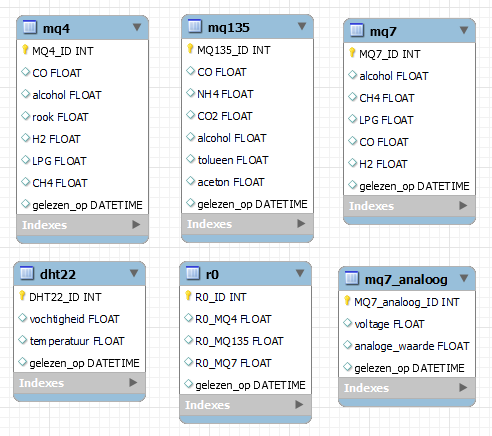
\includegraphics[scale=0.9, center]{SQLtabellen.png}
    \caption[Tabellen in de databank]{Tabellen in de MySQL databank}
    \label{fig:SQLtabellen}
\end{figure}

Deze databank wordt gehost met Apache, de ESP01 en de hostcomputer moeten dus op hetzelfde netwerk zitten. Hoe Apache werd ingesteld is te vinden in bijlage~\ref{sec:database}. Om de waarden daadwerkelijk in de databank te krijgen moet gebruik worden gemaakt van PHP scripts. In deze scripts wordt er een connectie gemaakt met de databank en worden de waarden via SQL-statements in de juiste tabel gegoten. In de volgende listing is een voorbeeld te zien van het PHP-script voor de gasmetingen van de MQ-135:
\begin{lstlisting}[language=PHP,caption={PHP-script MQ-135}]
<?php

$MQ135_CO_ppm = $_POST["MQ135_CO_ppm"];
$MQ135_NH4_ppm = $_POST["MQ135_NH4_ppm"];
$MQ135_CO2_ppm = $_POST["MQ135_CO2_ppm"];
$MQ135_alcohol_ppm = $_POST["MQ135_alcohol_ppm"];
$MQ135_tolueen_ppm = $_POST["MQ135_tolueen_ppm"];
$MQ135_aceton_ppm = $_POST["MQ135_aceton_ppm"];


$servername = "localhost";
$username = "root";
$password = "root";
$dbname = "db_arduino";

// Create connection
$conn = new mysqli($servername, $username, $password, $dbname);
// Check connection
if ($conn->connect_error) {
    die("Connection failed: " . $conn->connect_error);
}

$sql = "INSERT INTO MQ135 (CO, NH4, CO2, alcohol, tolueen, aceton, gelezen_op) VALUES ($MQ135_CO_ppm, $MQ135_NH4_ppm, $MQ135_CO2_ppm, $MQ135_alcohol_ppm, $MQ135_tolueen_ppm, $MQ135_aceton_ppm, NOW())";
if ($conn->query($sql) === TRUE) {
    echo "New record created successfully";
} else {
    echo "Error: " . $sql . " => " . $conn->error;
}


$conn->close();

?>

\end{lstlisting}

Als de databank is opgezet, de PHP-scripts zijn geschreven en Apache runt kunnen met behulp van de volgende AT-commando's waarden worden toegevoegd aan de databank:
\begin{lstlisting}[language=Java,caption={ESP01 naar de database}]
AT+CIPSTART="TCP","192.168.1.44",80  //lokale IP adres van de host
    CONNECT
    OK

AT+CIPSEND=236  //grootte van het bericht
    OK
    
> POST /insertMQ4DB.php HTTP/1.1    //naam php script
  Host: 192.168.1.44
  Connection: keep-alive
  Content-Type: application/x-www-form-urlencoded
  Content-Length: 86

  MQ4_CO_ppm=1&MQ4_alcohol_ppm=2&MQ4_rook_ppm=3&MQ4_H2_ppm=4&MQ4_LPG_ppm=5&MQ4_CH4_ppm=6

    SEND OK
    
    +IPD,285:HTTP/1.1 200 OK
    Date: Tue, 2 Apr 2024 14:54:11 GMT
    Server: Apache/2.4.58 (Win64) OpenSSL/3.1.3 PHP/8.2.12
    X-Powered-By: PHP/8.2.12
    Content-Length: 31
    Keep-Alive: timeout=5, max=100
    Connection: Keep-Alive
    Content-Type: text/html; charset=UTF-8
    New record created successfully

    CLOSED
    
\end{lstlisting}


\section{Implementatie van de warmte-koelcyclus}%
\label{sec:warmte_koel}


Zoals besproken in sectie~\ref{sec:warmte-koelcyclus} is het werkingsprincipe van de MQ-7 sensor anders dan de andere sensoren. Voor optimale resultaten moet er  gebruik worden gemaakt van een warmte-koelcyclus. In het onderzoek van 
%TODO calibrationandimplemantationofMQ7 pdf bron
wordt duidelijk uitgelegd hoe deze warmte-koelcyclus kan worden geïmplementeerd. 

In figuur~\ref{fig:heatcool_circuit} wordt aangetoond aan hoe het circuit diagram uit moet uit zien volgens %TODO calibrationandimplemantationofMQ7 pdf bron

\begin{figure}[h]
    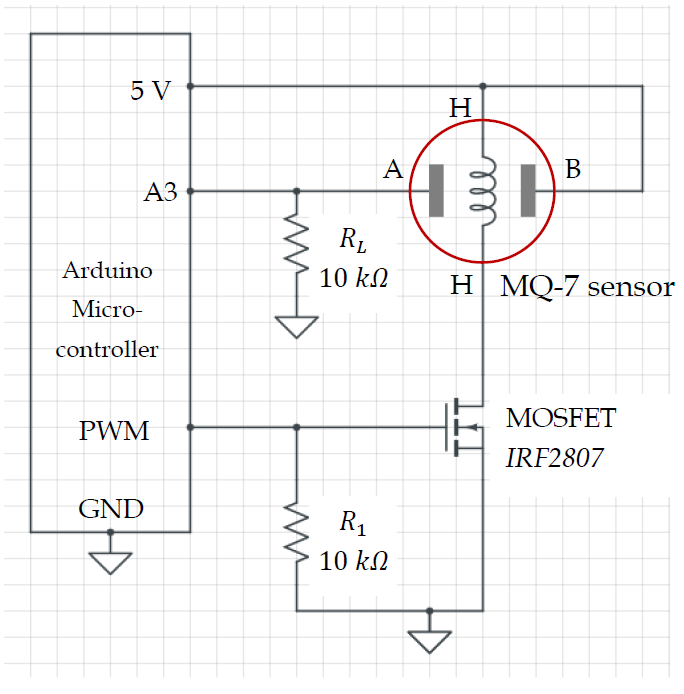
\includegraphics[scale=0.3, center]{heatcool_circuit.png}
    \caption[Circuit warmte-koelcyclus]{Het circuit voor een warmte-koelcyclus
    %TODO calibrationandimplemantationofMQ7 pdf bron
    }
    \label{fig:heatcool_circuit}
\end{figure}

In dit circuit is te zien hoe de opwarming van de MQ-7 sensor gebeurt, de Arduino stuurt de MOSFET transistor aan om zo het voltage van de MQ-7 te veranderen. De MQ-7 moet 60 seconden lang 5V toegediend krijgen om alle gassen te verdampen en de sensor te reinigen. In de tweede fase krijgt de sensor 90 seconden lang 1.4V toegediend, hier kunnen gassen opnieuw worden geabsorbeerd. De volgende listing toont aan hoe kan worden gedaan in Arduino code:

\begin{lstlisting}[language=Java,caption={Warmte-koelcyclus MQ-7}]
//pinnen vd sensoren 
int MQ7 = A2;
int mosfet = 9;

void setup() {
    Serial.begin(9600);
    pinMode(MQ7, INPUT);
    pinMode(mosfet, OUTPUT);
}

void loop() {
    // MQ7 hoog (voor 60 sec)
    analogWrite(mosfet, 255); //5V naar MQ7
    delay(60000);
    // MQ7 laag (voor 90 sec)
    analogWrite(mosfet, 72); //1.4V naar MQ7
    delay(90000);
    
    Serial.println(analogRead(MQ7));
}
        
\end{lstlisting}

Nu dit geïmplementeerd is kunnen deze waarden ook naar de database worden gestuurd voor een analyse. De grafiek (zoals bijvoorbeeld die van figuur~\ref{fig:mq7_heatcool_vb}) die ontstaat tijdens deze cyclus roept vragen op zoals: zijn verschillende gassen te onderscheiden in deze grafiek? En welke invloed heeft de temperatuur en vochtigheidsgraad?

\begin{figure}[h]
    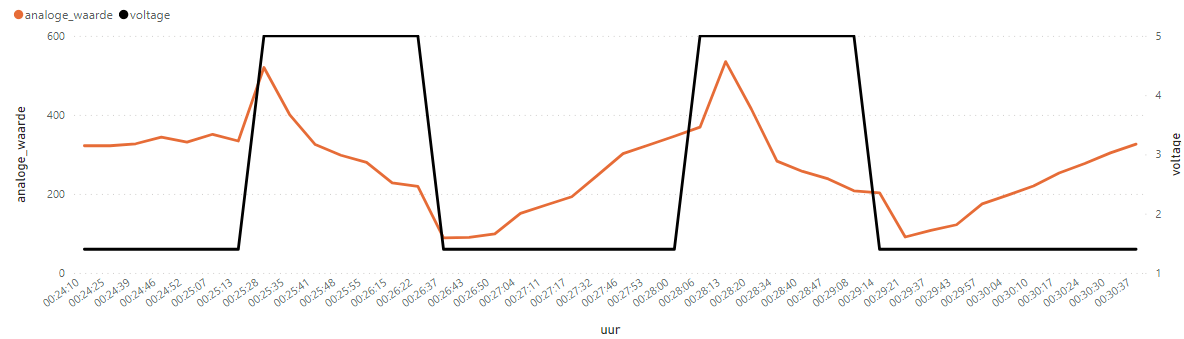
\includegraphics[scale=0.5, center]{mq7_heatcool_vb.png}
    \caption[Warmte-koelcyclus in de praktijk]{Voorbeeld van de visualisatie van de warmte-koelcyclus}
    \label{fig:mq7_heatcool_vb}
\end{figure}


Omdat dit interessante zaken kunnen zijn voor een analyse heb ik ze getest. Zo zijn er experimenten opgezet met 3 verschillende gassen waar de MQ-7 gevoelig voor is: CO, alcohol en LPG. Deze experimenten zijn uitgevoerd in een normale omgeving en een omgeving met een hoge vochtigheidsgraad.

%Een van de hoofdbestanddelen van rook is koolstofmonoxide, zo werd er door de rook van een brandende lucifer een hoge ppm CO gesimuleerd. Zo is er voor alcohol de damp van ontsmettingsalcohol gebruikt, en voor LPG de damp van aanstekerbenzine. De experimenten in normale omgeving werden buiten uitgevoerd, en voor de hoge vochtigheidsgraad is er in een vochtige badkamer gewerkt.

Omdat de ESP01 module niet snel genoeg data kan versturen, werd tijdens het experiment om de 2 seconden data geprint in de vorm van INSERT-statements in de Arduino IDE. Hierna kon deze output worden uitgevoerd in MySQL. Op deze manier is er meer detail uit te lezen op de grafieken. Deze resultaten worden besproken in sectie~\ref{sec:analyse_mq7}.




\section{Implementatie van de DHT22-sensor}%
\label{sec:dht22}


Om de DHT22-sensor te implementeren werd gebruik gemaakt van de DHT library op Arduino. Via deze library kan gemakkelijk de temperatuur en luchtvochtigheid worden afgelezen. De DHT22 is een stabiele en nauwkeurige sensor die geen kalibratie nodig heeft.

Om de correctiefactor te implementeren werd de werkwijze beschreven in sectie~\ref{sec:temp-en-hum} geïmplementeerd in de code. De volgende listing toont de functie bereken\_correctiefactor. Hier wordt er op basis van het sensortype, de temperatuur en de luchtvochtigheidsgraad berekent hoeveel de correctiefactor bedraagt.

\begin{lstlisting}[language=Java,caption={Berekenen van de correctiefactor}]
float bereken_correctiefactor(int sensor, float temp, float hum) {
    float y_33;
    float y_85;
    if (temp > 20) {
        switch (sensor) {
            case 4:
            y_33 = -0.00296 * temp + 1.05336;
            y_85 = -0.00434 * temp + 0.93704;
            break;
            case 7:
            y_33 = -0.00442 * temp + 1.08514;
            y_85 = -0.00398 * temp + 0.93537;
            break;
            case 135:
            y_33 = -0.00233 * temp + 1.02679;
            y_85 = -0.00273 * temp + 0.95286;
            break;
            default:
            Serial.println("Foute sensor");
            break;
        }
    } else {
        switch (sensor) {
            case 4:
            y_33 = 0.00022 * pow(temp,2) - 0.01178 * temp + 1.14896;
            y_85 = 0.00012 * pow(temp,2) - 0.00940 * temp + 0.99210;
            break;
            case 7:
            y_33 = 0.00046 * pow(temp,2) - 0.01945 * temp + 1.21352;
            y_85 = 0.00021 * pow(temp,2) - 0.01249 * temp + 1.02743;
            break;
            case 135:
            y_33 = 0.00046 * pow(temp,2) - 0.02907 * temp + 1.37849;
            y_85 = 0.00041 * pow(temp,2) - 0.02534 * temp + 1.24596;
            break;
            default:
            Serial.println("Foute sensor");
            break;
        }
    }
    return y_33 + ((y_85-y_33)/(85-33))*(hum-33);
}
\end{lstlisting}


\section{Finale code}%
\label{sec:final}

De finale code bestaat uit 4 scripts. In de eerste wordt de R\textsubscript{0} waarde berekent en naar de databank verstuurd (\ref{subsec:script_R0}), hier is de warmte-koelcyclus van de MQ-7 ook in opgenomen. In het tweede script wordt de data live naar Thingspeak geüpload (\ref{subsec:script_thingspeak}) en in het derde naar de databank (\ref{subsec:script_db}). Het vierde script werd gebruikt voor de testen met de MQ-7 sensor (\ref{subsec:script_mq7}).

Al deze scripts kunnen worden uitgevoerd met het circuit afgebeeld in figuur~\ref{fig:arduino_circuit}.

\begin{figure}[h]
    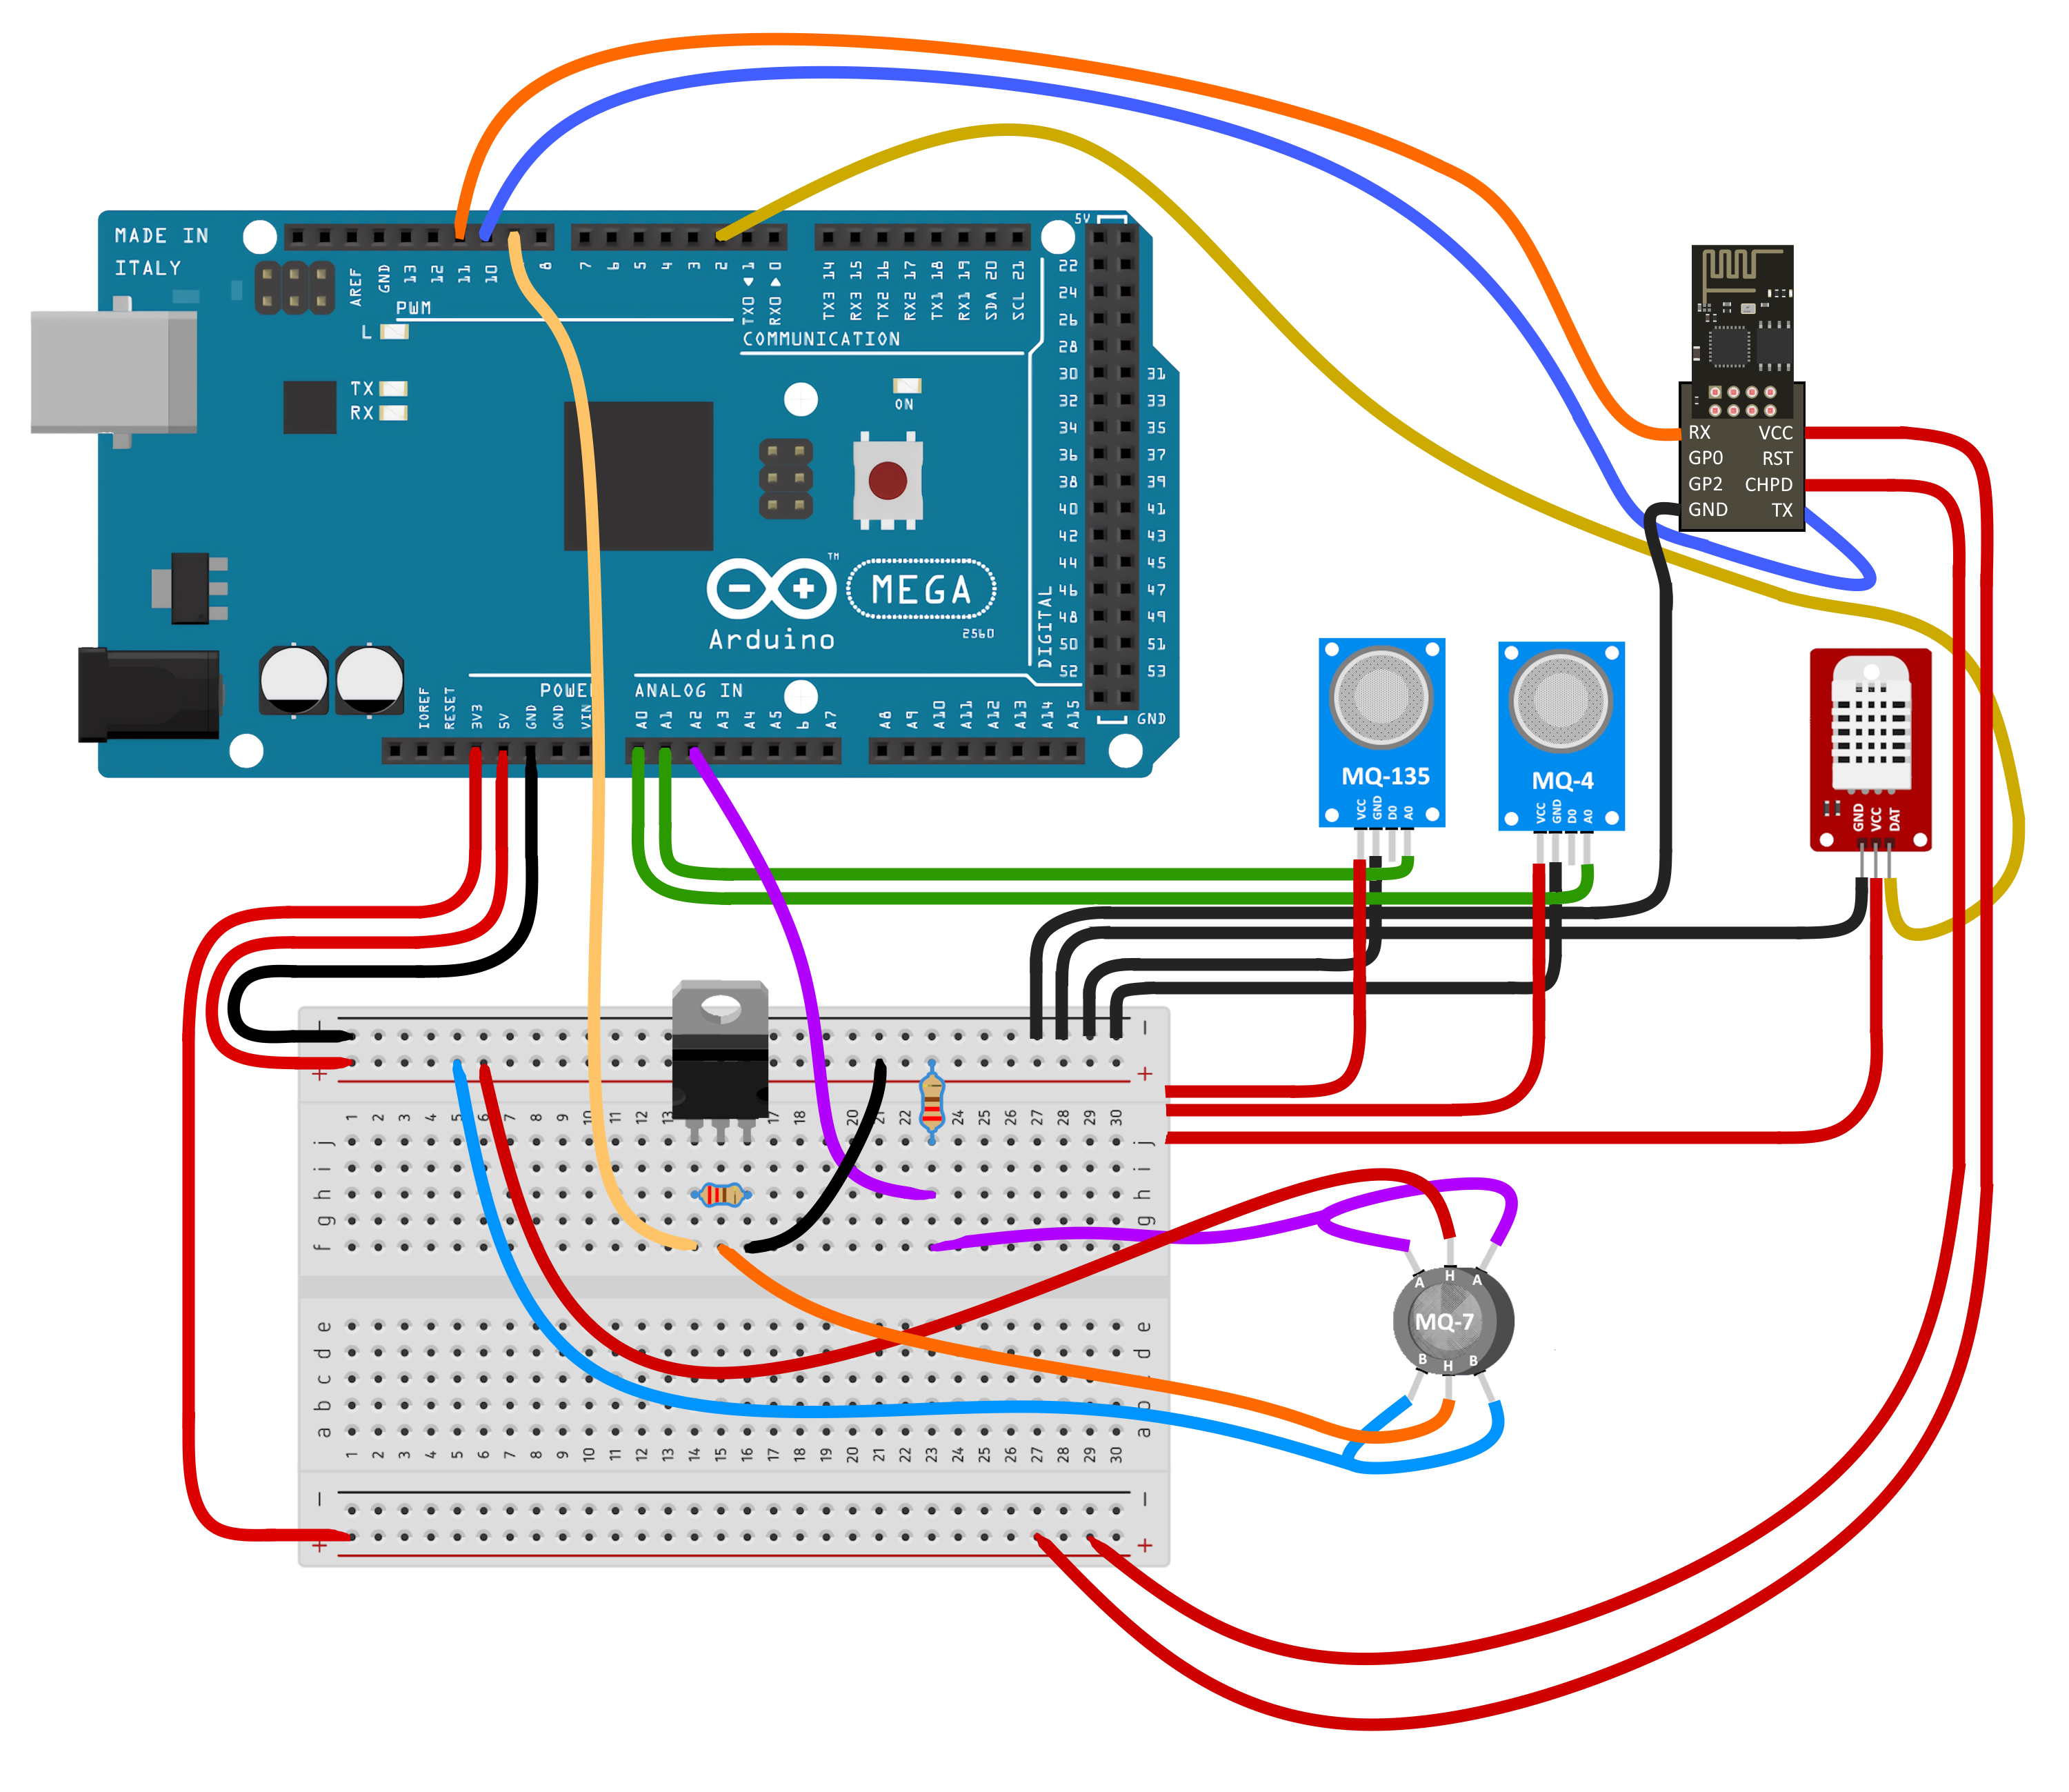
\includegraphics[scale=0.16, center]{arduino_circuit.png}
    \caption[Circuit test set-up]{Finale circuit van de test set-up}
    \label{fig:arduino_circuit}
\end{figure}

\begin{figure}[h]
    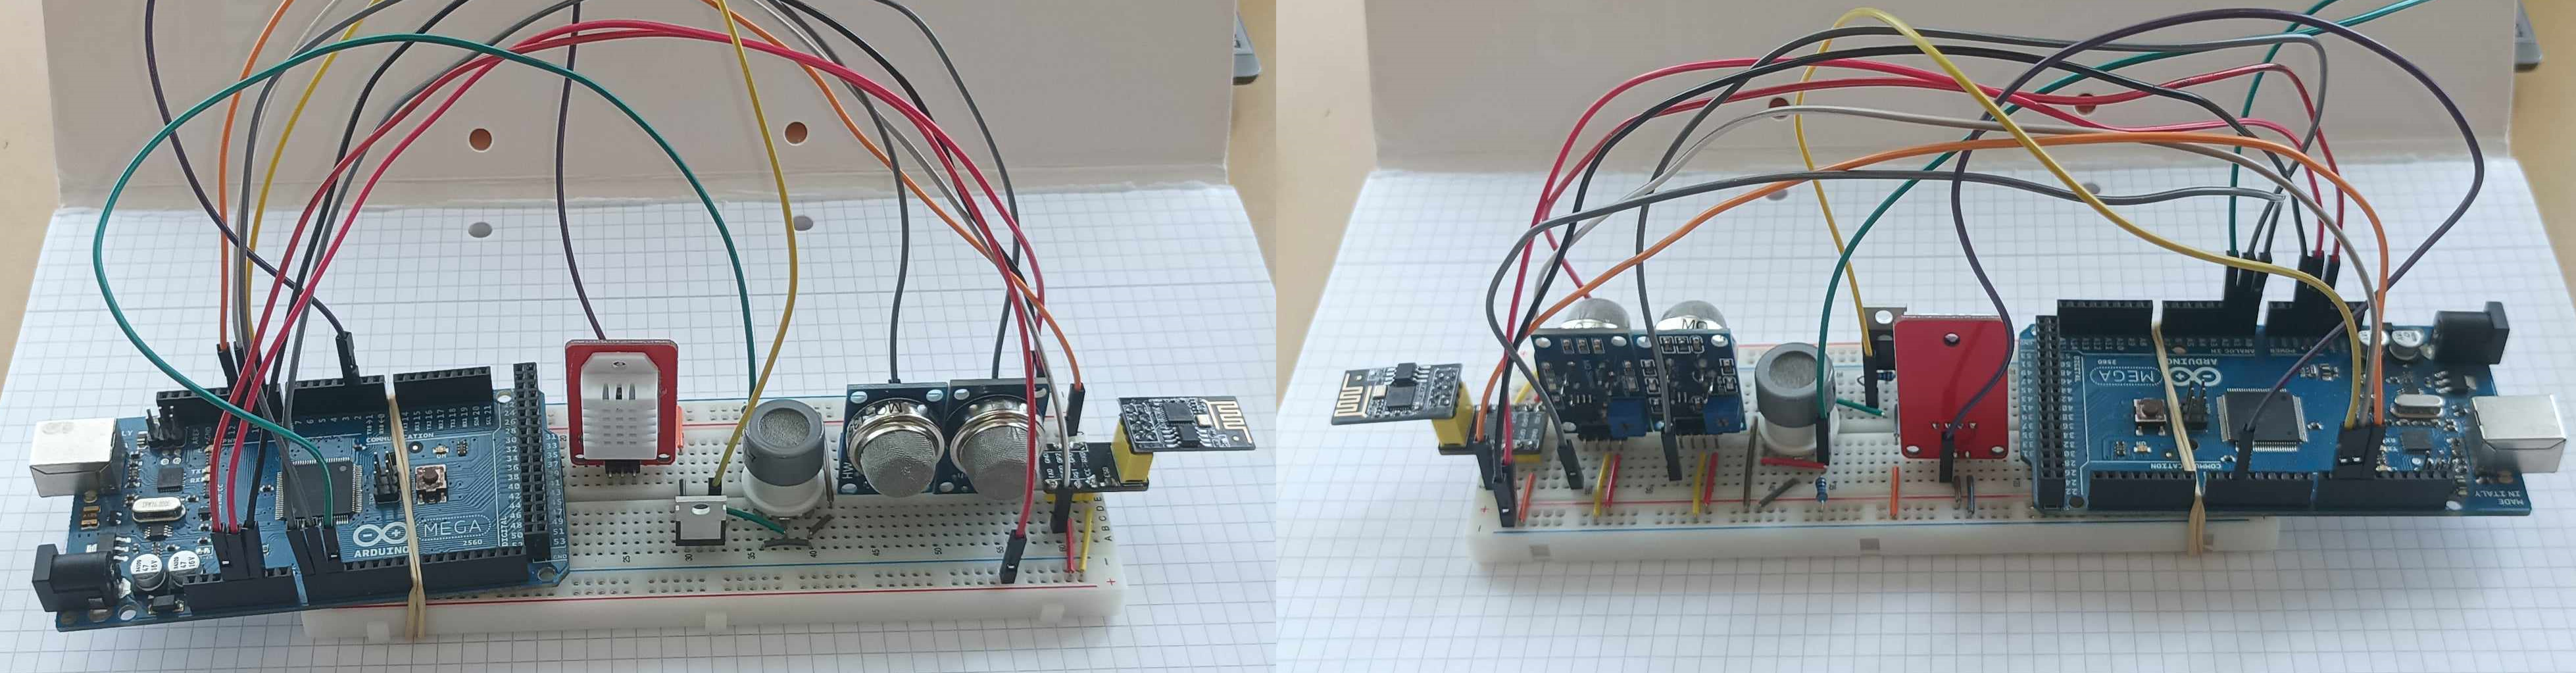
\includegraphics[scale=0.16, center]{voor_en_achterkant.png}
    \caption[Foto test set-up]{Voor- en achterkant van de test set-up}
    \label{fig:voor_en_achterkant}
\end{figure}


Deze test set-up werd uiteindelijk getest in een kalibratiesetup van ILVO. Hier worden andere gassensoren gekalibreerd die worden opgehangen in stallen, indien deze sensoren geen correcte resultaten geven kunnen ze zo worden bijgesteld. Zo zijn er 2 testen uitgevoerd, een met ammoniak en een met koolstofdioxide. Bij deze kalibratie zitten al de gassensoren in een luchtdichte kist waar gekende gasconcentraties naartoe worden gestuurd. Deze gasconcentraties worden terwijl ook geanalyseerd door een Picarro gassensor. Dit is een zeer nauwkeurige gassensor met een prijskaartje van 150.000€. De Picarro gassensor werkt op basis van een infraroodlaser en kan N\textsubscript{2}0, CH\textsubscript{4}, NH\textsubscript{3} en CO\textsubscript{2} meten.

In de eerste test werd NH\textsubscript{3} aangeboden, dit was interessant om te testen omdat NH\textsubscript{3} een veelvoorkomende en gevaarlijke stalgas is. In de gevoeligheidsgrafieken van de 3 MQ-sensoren staat geen NH\textsubscript{3}, zo werd dus getest of de sensoren daadwerkelijk geen NH\textsubscript{3} konden meten. En indien dit wel lukte, welke sensor hier het beste op reageerde. De NH\textsubscript{3} werd toegediend in 5 fases, in de eerste fase werd een halfuur lang niks aangeboden. Daarna werd 1, 3 en 5 ppm NH\textsubscript{3} per anderhalf uur toegediend. In de laatste fase werd terug voor een halfuur 0 ppm aangeboden om te testen hoe snel de sensoren terug zouden stabiliseren.

In de tweede test werd CO\textsubscript{2} aangeboden, hier werd vooral getest hoe accuraat de MQ-135 is die CO\textsubscript{2} meet. Maar ook werd getest hoe hard de andere sensoren hier op reageerden. In de beide testen werd de correctiefactor voor temperatuur en luchtvochtigheid apart opgeslagen om te zien hoe veel invloed dit had.

De resultaten van deze twee testen worden besproken in sectie~\ref{sec:nauwkeurigheid}.

\begin{figure}[h]
    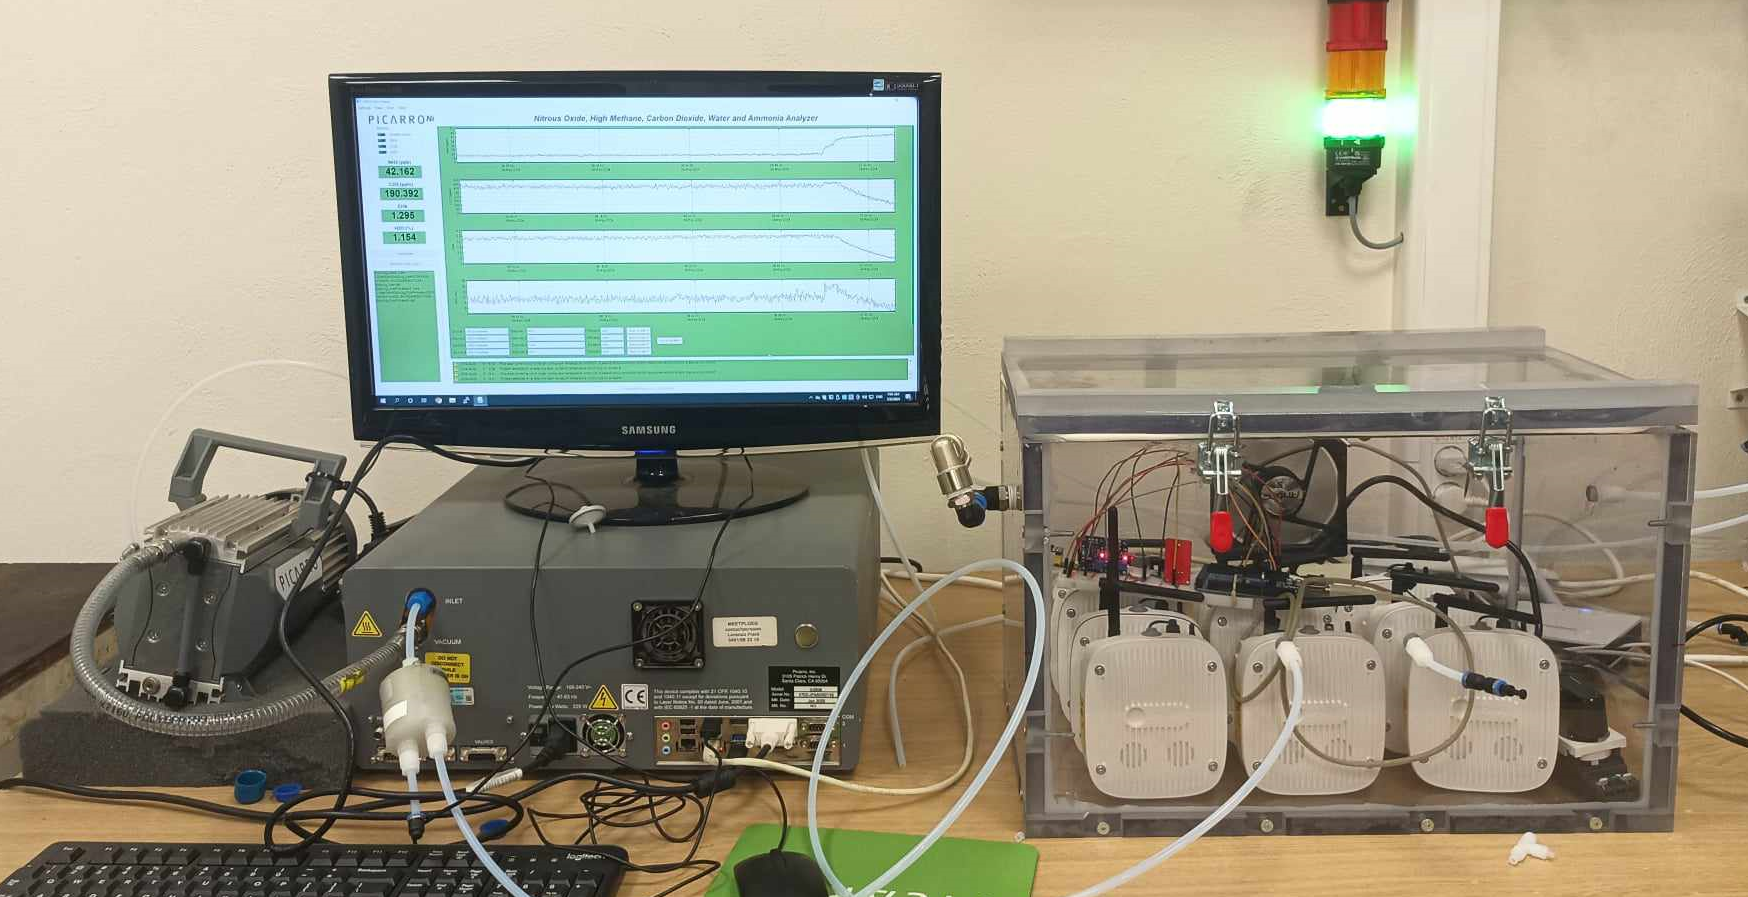
\includegraphics[scale=0.3, center]{test.png}
    \caption[Kalibratiesetup]{De complete kalibratiesetup bij ILVO met de Picarro gassensor (links) en de luchtdichte kist met de andere gassensoren (rechts)}
    \label{fig:test}
\end{figure}








